\documentclass[12pt,fleqn]{article}
\setlength{\parindent}{0pt}
\usepackage{graphicx}
\usepackage{listings}
\usepackage[latin5]{inputenc}
\setlength{\parskip}{8pt}
\setlength{\parsep}{0pt}
\setlength{\headsep}{0pt}
\setlength{\topskip}{0pt}
\setlength{\topmargin}{0pt}
\setlength{\topsep}{0pt}
\setlength{\partopsep}{0pt}
\setlength{\mathindent}{0cm}

\begin{document}
MIT OCW Cok Degiskenli Calculus - Ders 9

Bu dersin konusu birden fazla degisken iceren fonksiyonlarin minimizasyonu
ile ugrasirken yardimci olacak kismi turev (partial derivative)
kavrami. Cok degiskenli bir fonksiyon $f(x,y)$'nin birden fazla turevi
vardir. Mesela bunlardan bir tanesi

\[ \frac{\partial f}{\partial x} = f_x \]

Bu turev $x$'in degistirildigi ama $y$'nin sabit tutuldugu bir durumu
gosterir. 

\[ \frac{\partial f}{\partial y} = f_y \]

ise $y$'in degistirildigi ama $x$'nin sabit tutuldugu bir durumu gosterir.

Simdi her ikisinin birden degistirildigi durumda ne olacagini gosteren
yaklasiksal (approximate) formulu gorelim. Degisim matematiksel olarak
soyle

\[ x \sim x + \Delta x \]

\[ y \sim x + \Delta x \]

O zaman $z$ icin

\[ z = f(x,y) \]

yaklasiksal degisim soyle olur

\begin{equation}\label{eq1}
\Delta z \approx f_x\Delta x + f_y \Delta f_y
\end{equation}


Tekrar vurgulamak gerekirse bu yaklasiksal bir formul, daha ``dogru'' bir
temsil icin 2., 3. turevleri iceren daha yuksek dereden (higher order
terms) terimlerin de olmasi gerekir, fakat bu terimler 1. derece lineer bir
yaklasiksallik icin kullanilmaz. 

Bu formulu nasil dogrulariz? Bunu yapmanin yollarindan biri teget duzlem
yaklasiksallamasi (tangent plane approximation). Mesela $z = f(x,y)$
fonksiyonuna olan teget bir duzlemi dusunelim.

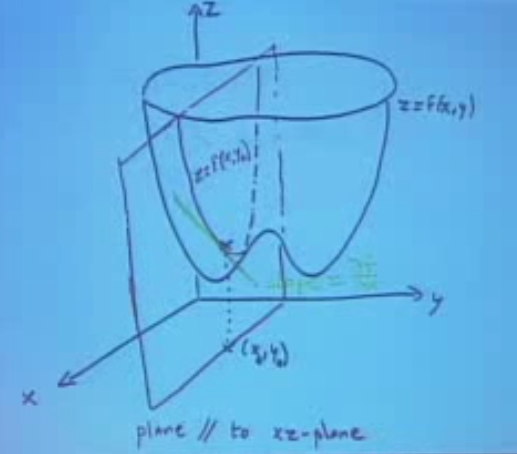
\includegraphics[height=4cm]{9_1.png}

Hatirlarsak $\frac{\partial f}{\partial x}$ kismi turevi $x$'in degistigi
ama $y$'nin sabit tutuldugu bir durumu tarif ediyordu. Yukaridaki grafige
gore bu bir anlamda iki cukurlu kap gibi duran $z$ fonksiyonun bir kesitine
bakmak gibi (unutmayalim, fonksiyon sadece kabin disinda tanimli, ici
bos). Bu kesit uzerine $f$'in bir yansimasi olusuyor, o yansima ustteki
grafikte bir parabol seklinde. Bu parabolda $x$ degistikce o noktanin
parabol uzerindeki cizgizel tegeti de degisiyor (grafikteki yesil cizgi) ki
bu cizgisel egim $\frac{\partial f}{\partial x}$'e esit.

Eger ayni seyi $x$'in sabit $y$'nin degistigi durum icin yapsaydim,
benzer bir kesit elde edecektim. 

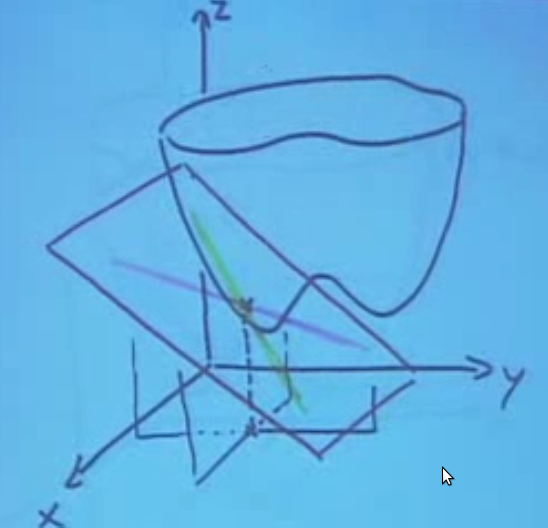
\includegraphics[height=4cm]{9_2.png}

Bu iki kesit uzerinden elde edilen ikinci teget cizgi birinci ile beraber
kullanilinca bir duzlemi tanimlamak icin kullanilabilir (iki cizgi paralel
bir duzlem tanimlamak icin yeterlidir), ki teget duzlem yaklasiksallamasi
icin kullanilacak duzlem budur. Formulsel olarak bunu nasil yapacagimizi
gosterelim.

$f_x$ ve $f_y$ iki teget cizgiyi tanimlamak icin kullaniliyorsa, bu
formulleri bir araya koyarak duzlemi temsil edebilirim. Eger

\[ \frac{\partial f}{\partial x}(x_0,y_0) = a \]

ise bu demektir ki birinci teget cizgi (yesil cizgi) $L_1$ soyledir:

\[ 
L_1 = 
\left\{ \begin{array}{l}
z = z_0 + a(x - x_0) \\
y = y_0
\end{array} \right.
 \]

Bu cizgi icin $y$'yi sabit tutuyorum, $z$'deki degisimi $z_0$ ustune egim
$a$'nin katlari kadar ($x$'in degisimi oraninda carparak) ekleyerek
hesapliyorum. 

Benzer sekilde

\[ \frac{\partial f}{\partial y}(x_0,y_0) = b \]

\[ 
L_2 = 
\left\{ \begin{array}{l}
z = z_0 + b(y - y_0) \\
y = y_0
\end{array} \right.
 \]

Hem $L_1$ hem de $L_2$ $z = f(x,y)$'ye tegettir. Bu iki cizgi beraber bir
duzlem olusturur. Bu formul

\begin{equation}\label{eq2}
z = z_0 + a(x-x_0) + b(y-y_0) 
\end{equation}

formuludur. 

Formul \ref{eq1}, ustteki formulun yaklasiksal halidir. Eger teget duzlem
uzerinde olsaydik, $\approx$ isareti $=$ isaretine donusecekti. Bu
yaklasiksallik ufak $\Delta x$ ve ufak $\Delta y$ icin gecerli. Yani
yaklasiksal formul, $f$'nin grafigi teget duzleme yakin diyor. 

Maksimum Minimum Problemleri 

Kismi turevlerin kullanim alanlarindan biri optimizasyon
problemleridir. Mesela cok degiskenli bir fonksiyonun maksimumunu bulmak
gibi. Eger fonksiyon tek degiskenli olsaydi, hemen turevini alip sonucu
sifira esitleyebilirdik, ve buna gore bir cozum arardik. Cok degiskenli
fonksiyonlarda kismi turevler kullanmak lazim. 

Bu derste iki degiskenli duruma bakacagiz fakat ayni prensipler, 10, 15,
milyon tane degisken icin ayni. 

Lokal bir minimum icin hem $f_x=0$ hem $f_y=0$ olmalidir. Bu niye
dogudur? Yine formul \ref{eq1}'e bakarsak, hem $f_x=0$ hem $f_y=0$ oldugu
zaman $\Delta z$ sifir olacaktir, yani birinci derecede dusunursek
$f(x,y)$'de degisim yok demektir. 

Teget duzlemlerin dilinden konusursak, minimum aninda teget duzlem tamamen
yatay olacaktir. 

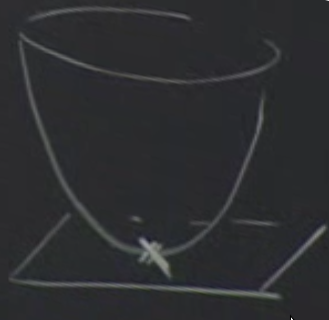
\includegraphics[height=3cm]{9_3.png}

Formul \ref{eq2} baglaminda dusunursek, bu durum $a=0$ ve $b=0$ oldugu ana
tekabul ediyor ve o anda duzlemi tanimlayan $z = z_0$ formuludur. 

Tanim

Eger $f_x(x_0,y_0)= 0$ ve $f_y(x_0,y_0)= 0$ ise o zaman $x_0,y_o$ $f$'in
kritik noktasidir. Not: Birden fazla degisken icin tabii ki tum kismi
turevlerin o noktada sifir olmasi gerekir.

Ornek

\[ f(x,y) = x^2 - 2xy + 3y^2 + 2x - 2y \]

Bakalim bunu minimize ya da maksimize edebilecek miyiz? 

\[ f_x = 2x - 2y + 2 = 0\]

\[ f_y = -2x + 6y - 2 = 0 \]

Ustteki iki denklemi ayni anda cozmeliyiz. 

Bu tur durumlarda iki denklemi birbiriyle toplayip basitlestirmeye calismak
iyi bir yontemdir. Fakat unutmayin, elimizde her zaman iki tane denklem
olmali, iki denklemi ortadan kaldirip birdenbire tek denklem ile yola devam
edemeyiz. 

Toplami yaparsak

\[ 4y = 0 \]

elde ederiz. Bunu alip birinci denkleme sokalim, sonuc

\[ 2x + 2 = 0 \]

\[ x = -1 \]

Demek ki kritik nokta $(x,y) = (-1,0)$. 

Peki bu kritik noktanin minimum mu maksimum mu oldugunu nereden bilecegiz?
Eger tek degiskenli bir fonksiyona bakiyor olsaydik, ikinci tureve
bakabilirdik. Benzer bir seyi burada da yapabilirdik, ama sadece birinci
turevden bile elimizde iki tane var, ikinci turevlerden cok daha fazlasi
olacak. O duruma bakacagiz, simdilik daha az otomatik olarak isi nasil
anlayacagimizla ilgilenelim. 

Elimizde birden fazla minimum olabilir. Turev(lerin) sifir oldugu noktada
bir duzluk vardir, bu bir lokal minimumdur. Yani o noktaya yakin oldugumuz
surece (ki lokalligin tanimi bu) bu minimum gecerlidir. Baska bir noktada,
turev(lerin) yine sifir oldugu ama daha asagi noktada bir minimum daha
olabilirdi. Maksimumlar icin ayni durum gecerli.

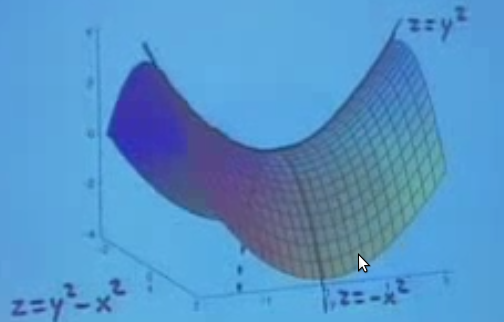
\includegraphics[height=4cm]{9_4.png}

Yanliz bir diger secenek daha var. Bu secenek kritik noktanin ne maksimum,
ne minimum oldugu durumdur. Bu durumda kritik noktadan hangi ``yone dogru''
bakiyorsak, degisik bir cevap elde ederiz. Bu at egeri gibi gozuken
grafigin orta noktasina, 0,0,0 noktasina bakalim, burada teget duzlem tam
yatay. Bu noktaya eger noktasi (saddle point) deniyor. Eger $z=y^2$ yonune
dogru bakarsak min durumdayiz, eger $z=-x^2$ yonune dogru bakarsak maks
durumdayiz. 

2. turevlerden bahsetmisik, ve bu derste kritik noktanin ne oldugunu daha
az otomatik bulacagimizi soyledik (2. turevler bir dahaki derste). 

Bu yontemde kareler kullanacagiz. Niye kareler? Cunku karesel ifadeler en
az sifir olabilirler -- bir deger ne olursa olsun, eksi bile olsa karesi
alinirsa arti olur, ve bu tur ifadeler sadece sifirda ``en az'' olurlar.

O zaman $f(x,y)$'i karelerin toplami olarak tekrar temsil etmeye
ugrasalim. $f(x,y)$'de zaten kareler var ama tum formulu bir seylerin
karesi olarak gosterebilirsek, hedefimize erisebiliriz. Tek problem $xy$
terimi, ama $x^2 - 2xy..$ diye giden bir baska formul biliyoruz, Kareyi
Tamamlama ile onu kullanalim.

\[ f(x,y) = (x-y)^2 + 2y^2 + 2x - 2y \]

Basitlesti ama biraz daha basitlesebilir. Acaba $(x-y)^2$ icindeki $(x-y)$
ile disaridaki $2x - 2y$ arasindaki bir baglanti kurabilir miyiz? Iceriye
bir +1 eklersek bu olabilir, o zaman disaridaki $2x - 2y$ iptal
olur. Icerideki 1'i dengelemek icin ise disari bir -1 ekleriz.

\[  = ((x-y) + 1)^2 + 2y^2 - 1\]

Iste, tum formul artik karelerden olusuyor. Bu formul eger 

\[  = \underbrace{((x-y) + 1)^2}_{\ge 0} + \underbrace{2y^2}_{\ge 0} - 1\]

ise ancak $\ge -1$ olabilir. Ve kritik nokta (-1,0)'da $f$'in degeri
hakikaten -1'dir. Ustteki iki terimin niye $\ge 0$ oldugundan
bahsettik. Demek ki bu nokta bir minimum.  Yani biraz cebirsel takla, ve
ufak bir numarayla istedigimiz sonuca erismis olduk.

Simdi min/maks probleminin ilginc bir uygulamasini gorelim. Bu uygulamayi
min/maks kategorisinde gormeyebilirsiniz, ama aslinda problem min/maks ile
cok guzel bir sekilde cozuluyor.

Deneysel bilimlerde en az karelesel interpolasyon (least squares
interpolation) adli bir teknik kullanilir. Mesela bir deney yapariz, ve
deneyden gelen verileri aliriz. Mesela kurbagalari inceliyoruz, ve kurbaga
bacak uzunlugunu kurbaga goz buyuklugu arasinda bir baglanti ariyoruz. Ya
da baska bir seyi olcuyoruz, genel olarak bir $x$ degiskeni icin onun etki
ettigi, alakali oldugu bir $y$ degiskenini olcuyoruz.

Olculen iki degiskeni grafikleyince, su ortaya cikiyor diyelim.

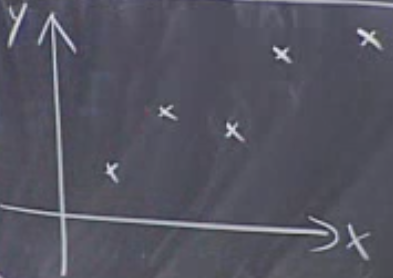
\includegraphics[height=3cm]{9_5.png}

Arada bir korelasyon oldugunu goruyoruz. Bu konu hakkinda bilimsel bir
makale yaziyor olsaydik, bu grafikte soyle bir cizgi cizerdik, 

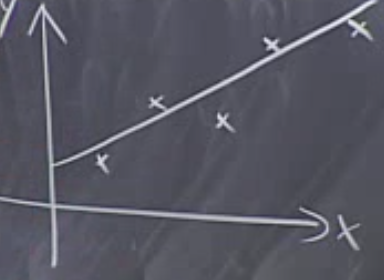
\includegraphics[height=3cm]{9_6.png}

Fakat veri noktalarinin tam ortasindan gecen bu cizgiyi nasil cizecegiz?
Yani cozmek istedigimiz problem verilen $(x_1,y_1), (x_2,y_2),...(x_n,y_n)$
seklindeki deney verileri icin ``en iyi uyan (best fit)'' cizgi $y=ax + b$,
en iyi yaklasiksallik nedir? 

Bu problemde onemli bir puf noktasina isaret edelim: $y=ax + b$ denkleminde
bilinmeyenler nedir? Genellikle ogrenciler $x$ ve $y$ degiskenine
bakiyorlar. Fakat bu dogru degil. Bir optimal cizgi ortaya cikarmak
istiyorsak ilgilendigimiz $x$ ve $y$ degil, esas ilgilendiklerimiz $a$ ve
$b$ katsayilari. Cizginin hangi sekilde oldugunu onlar kontrol ediyorlar,
yani dogru uyum icin cizginin nereden gectiginin hesaplanmasi problemindeki
bilinmeyenler onlar. Yani uyum icin en iyi $a$ ve $b$'yi bulmamiz
gerekiyor.

Bu noktada ``en iyi $a$ ve $b$'' ifadesinin ne olduguna karar vermemiz
lazim. En iyi, $a$ ve $b$'nin bir fonksiyonunun minimize edilmesi olabilir,
ki bu fonksiyon deneysel veri ile bir teorik cizgi arasindaki uyum
hatalarinin toplamini temsil edebilir. Yani hata, o cizginin deney
noktalarindan ne kadar uzakta oldugunun toplami ile temsil edilebilir.

``Uzakligi'' hesaplamanin da degisik yollari olabilir. Mesela her noktanin
bir cizgiye olan duz uzakligi olculebilir. Ya da deneysel noktadan dikey
olarak yukari / asagi cikip cizgiye gelinceye kadar olan uzaklik. Ya da
uzakligi en fazla olan tek noktanin mesafesi azaltilmaya ugrasilabilir (ama
bu son yontem pek iyi bir secim olmayabilir, cunku belki deney sirasinda
uykuya dalmissinizdir, ve cok yanlis bir nokta olcmussunuzdur, ve o nokta
tum uyum hesabini bozukluga ugratir).

Bu tur seceneklerden bir tanesi en iyisidir, ve evrensel olarak kullanilan
yaklasim da o'dur. En Az Kareler demistik, bu yontemde hata noktalarin
cizgiye olan uzakliklarin karesinin toplamidir. Bu yontem iyi sonuclar
veriyor ve hesap icin oldukca temiz bir formul ortaya cikartiyor. Demek ki
``en iyi'' tanimi hata noktalarin cizgiden olan sapmasinin karesinin
toplaminin minimize edilmesi demek. Sapma nedir? Tahmin edilen ile gercek
veri noktasinin farkidir. 

\[ y_i - (ax_i + b) \]

O zaman problem

\[ \textrm{Minimize Et } D = \sum_{i=1}^n \bigg[ y_i - (ax_i+b) \bigg]^2 \]

Tekrar vurgulayalim, bu fonksiyonda bilinmeyenler $a$ ve $b$. $x_i$ ve
$y_i$ deneyden gelen veriler. 

Minimize etmek icin simdiye kadar ogrendiklerimizi kullanabiliriz. Kritik
noktayi bulalim. 

Yani istedigimiz 

\[ \frac{\partial D}{\partial a} =0 \]

\[ \frac{\partial D}{\partial b} =0 \]

esitliklerini dogru oldugu an. Kritik nokta burada. Kismi turevleri alalim.

\[ \frac{\partial D}{\partial a}  =
\sum_{i=1}^n 2 (y_i (ax_i+b)) (-x_i) 
= 0
 \]

\[ \frac{\partial D}{\partial b} = 
\sum_{i=1}^n 2 (y_i (ax_i+b)) (-1) 
=0 \]

Cozmemiz gereken denklemler bunlar. 

Eger dikkat edersek bu denklemler $a$ ve $b$ baglaminda
lineer. Denklemlerde biraz kalabaliklik var, onlari acip tekrar
duzenleyerek bu lineerligi gormeye ugrasalim. 

Ilk once '2' terimini atalim, ona gerek yok. Iki denklem ayri ayri soyle
olur:

\[ \sum_{i=1}^n (x_i^2a + x_ib - x_iy_i) = 0\]

\[ \sum_{i=1}^n (x_i^2a + b - y_i) = 0\]

$a$ ve $b$ leri yanyana getirelim. Yine ayri ayri

\[  \bigg(\sum_{i=1}^n x_i^2\bigg)a + \bigg(\sum_{i=1}^n x_i\bigg) b = \sum_{i=1}^n x_iy_i\]

\[  \bigg(\sum_{i=1}^n x_i\bigg)a + nb = \sum_{i=1}^n y_i \]

Parantezler icindeki $x_i$'li ifadeler korkutucu gorunuyor olabilir, fakat
bunlar deney verisinden gelen sayilarin toplamindan ibaret, onlar elimizde
sayisal olarak mevcut zaten. Deney verisini alip, hepsini toplayinca bu
sayiyi elde edecegiz. 

Sonuc olarak elimize gecen 2 x 2 boyutlarinda bir lineer sistem. Yani $x_i$
ve $y_i$ iceren ifadeleri hesapladigimiz anda bu sistemi elde ederiz, ve 2
x 2 bir lineer sistemi cozmeyi zaten biliyoruz. Ve kritik noktayi boylece
elde ederiz. Bir sonraki derste gorecegimiz 2. kismi turevleri kullanacagiz
yontemle de bu noktanin min/maks oldugunu anlariz. Bu testi uygulasak
ustteki yontemin hakikaten bir min urettigini gorebilirdik. 

En Az Kareler interpolasyonu cok daha genel kullanimlarda da ise yarar. 

Ornek

Bilgisayar dunyasinda Moore Kanunu denen bir kural vardir, bu kural
bilgisayar ciplerinin nasil surekli daha hizli, daha iyiye dogru gittigini
anlatir. Unlu cip ureticisi Intel baskani Andy Grove tarafindan ortaya
atilmistir, bir hipotezdir, fakat sasirtici bir sekilde dogru
cikmistir. Kuralin olctugu bir mikropcipin icine koyulabilecek transistor
sayisidir. Bu olcumun bir ornegi alttadir. 

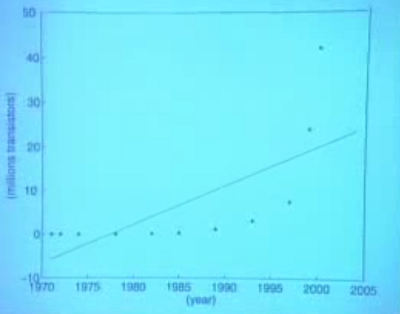
\includegraphics[height=4cm]{9_7.png}

Bu veriye lineer olarak uyum yapamazdik. Fakat logaritmik skalayi
kullanirsak, yani transistor sayisi yerine onun logaritmasini alip
grafiklersek, 

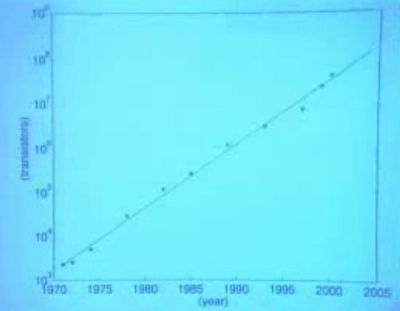
\includegraphics[height=3cm]{9_8.png}

veriler daha cizgisel olurlar. Bu demektir ki zaman ve transistor sayisi
arasindaki iliski ustel (exponential) bir iliskidir. Zaten kuralin
soyledigi de bu, kural her 18 ayda bir cip icindeki transistor sayisinin
ikiye katlandigini soyler. Bir sonraki buyuklugun o buyuklugun o anki
halinin belli bir kati olmasi (aynen nufus artisinda oldugu gibi) ustel bir
iliskiye isaret eder. 

Peki en iyi ustel uyumu nasil buluruz? Boyle bir uyumun formulsel hali
sudur. Duz cizgi formulu yerine bir ustel ifade icerir. 

\[ y = ce^{ax} \]

Fakat bu formulu direk hata hesabinda kullanirsak, ele gecen formuller cok
karmasik hale geliyor. Ama ustteki numarayi hatirlayalim, log skalasinda
bakinca her sey lineer cikiyor. O zaman uyumu su sekilde yapabiliriz,
ustteki formulun log'unu alalim:

\[ ln(y) = ln(c) + ax \]

ki bu formul lineerdir. Bunun uzerinde En Az Kareler yontemini
kullanabiliriz. 

Ustel iliski yerine karesel bir iliski de olabilirdi, mesela

\[ y = ax^2 + bx + c \]

o zaman en iyi parabolu uydurmaya ugrasiyor olabilirdik, bu uyum icin $a$,
$b$ ve $c$'yi bulmamiz gerekirdi. Yani sunu minimize edecektik:

\[ D(a,b,c) = \sum_{i=1}^n (y_i - ( ax_i^2 + bx_i + c ))^2  \]

Burada kismi turevler 3 tane ayri denklem uretir, ve iliski yine lineer
cikar, 3 x 3 boyutunde bir sistem elde ederiz. 

Yani soyledigimiz gibi, bu problemler ilk basta minimizasyon problemi gibi
gozukmeyebiliyordu, ama oyle olduklarini simdi gormus olduk. 



\end{document}
